\chapter{Introdução}

Os motores BLDC (\textit{Brushless Direct Current Motor}) representam um avanço significativo em relação aos motores CC tradicionais porque eliminam a necessidade de escovas mecânicas para a conversão de energia, resultando em maior rendimento energético, menos desgaste e maior vida útil \cite{hanselman2003brushless}. Esses avanços tecnológicos estão sendo impulsionados pela crescente demanda por sistemas de acionamento de maior rendimento, confiáveis e de baixa manutenção em diversas aplicações industriais, comerciais e de consumo. A precisão e controlabilidade dos motores BLDC os tornam ideais para aplicações que exigem alta exatidão de movimento, velocidade e controle de torque, como robótica, automação industrial, veículos elétricos e eletrônicos de consumo.

\section{Objetivos}
Estudar o princípio de funcionamento de um controlador de motores Brushless, tornando possível o projeto e desenvolvimento de um protótipo que possa oferecer uma operação suave e precisa em diferentes cenários de aplicação.



\section{Motores CC Sem Escova}
O princípio de funcionamento dos motores BLDC é baseado em campos magnéticos gerados por ímãs permanentes e enrolamentos de  (Figura \ref{fig:motor-dc-bldc-comparativo}). A comutação da corrente para gerar movimento ocorre eletronicamente, por meio de um controlador dedicado normalmente chamado de ESC (Eletronic Speed Controller), que pode usar ou não sensores durante o processo, eliminando assim a necessidade de escovas mecânicas utilizadas em motores DC tradicionais. Esta abordagem resulta em uma diminuição significativa do desgaste mecânico, aumentando a vida útil do motor e reduzindo a necessidade de manutenção. Os motores BLDC são amplamente utilizados em uma variedade de aplicações, desde eletrônicos de consumo, como ventiladores e ferramentas elétricas, até aplicações industriais e automotivas. Sua capacidade de fornecer um controle preciso de velocidade e posição, juntamente com uma resposta rápida, faz deles a escolha ideal para sistemas que exigem rendimento energético e alta performance.

\begin{figure}[htbp]
	\centering
	\caption{Configuração de um motor DC convencional (A) e motor BLDC (B).}
	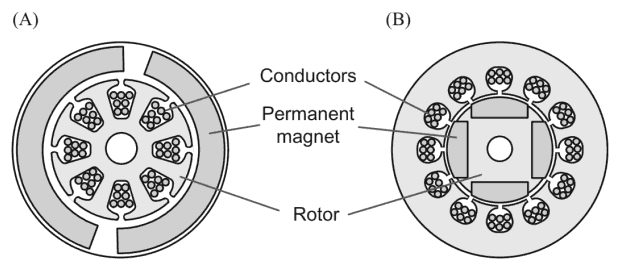
\includegraphics[width=8cm]{imagens/Comparativo.png}
	\legendafonte{\cite{kim2017electric}.}
 \label{fig:motor-dc-bldc-comparativo}
\end{figure}

Apesar das muitas vantagens, eles não estão isentos de algumas limitações. A complexidade eletrônica necessária para o controle preciso, o custo inicial potencialmente mais elevado comparado a motores elétricos escovados, a sensibilidade a ambientes de alta temperatura, pois podem gerar a desmagnetização dos imãs permanentes, a exigência de eletrônica de controle especializada, o potencial de ruído eletromagnético (EMI) e a complexidade de manutenção do sistema como um todo são fatores a serem considerados ao escolher essa tecnologia. Cada aplicação específica deve ponderar essas considerações em relação aos benefícios que os BLDC oferecem, como rendimento, durabilidade e controle superior.

São categorizados como síncronos, ou seja, o rotor gira na mesma frequência do campo magnético gerado pelo estator \cite{jahns1984torque}. Também não apresentam o fenômeno de escorregamento que é característico dos motores de indução. Os motores BLDC estão disponíveis em configurações de uma fase, duas fases e três fases, sendo  essa a mais amplamente utilizada, por serem equilibrados em relação a oscilação de torque e custo de construção \cite{hendershot1994design}.

A nomenclatura "Brushless DC" pode gerar uma interpretação equivocada. Embora alimentado por uma fonte de corrente contínua (DC), o motor BLDC é, em sua essência, um motor síncrono de ímãs permanentes (PMSM) \parencite{maquinasEletricasFitzgerald}. A rotação é induzida por campos magnéticos girantes gerados nos enrolamentos do estator, que são alimentados por formas de onda de corrente alternada (AC) sintetizadas por um controlador eletrônico. Portanto, a designação "DC" refere-se à fonte de alimentação externa, e não ao princípio físico de operação interna, que requer uma lógica de controle sofisticada para operar \parencite{ti2013sensorless}.

Nesse contexto, a performance do sistema é governada por parâmetros intrínsecos que descrevem a física da conversão de energia. Duas das mais importantes dessas constantes são a \textbf{constante de torque ($K_T$)} e a \textbf{constante de velocidade ($K_V$)}. Estes parâmetros são a manifestação matemática dos princípios físicos que regem a interação entre os domínios elétrico e mecânico do motor.

\subsection{Fundamentos Físicos da Conversão Eletromecânica}

A operação de um motor elétrico é governada por dois princípios físicos interligados: a Força de Lorentz, que gera o torque, e a Lei da Indução de Faraday, que gera uma força contraeletromotriz.

\subsubsection{A Força de Lorentz e a Condição de Torque Máximo}

A produção de força mecânica em um motor origina-se na Força de Lorentz. Esta lei descreve a força ($\vec{F}$) sobre um condutor de comprimento vetorial ($\vec{L}$) percorrido por uma corrente ($I$) e imerso em um campo magnético ($\vec{B}$). A relação vetorial é:
\begin{equation}
    \vec{F} = I \cdot (\vec{L} \times \vec{B})
\end{equation}
A magnitude desta força, $F = I \cdot L \cdot B \cdot \sin(\theta)$, onde $\theta$ é o ângulo entre o condutor e o campo magnético, é maximizada quando $\sin(\theta) = 1$, o que ocorre precisamente quando $\theta = 90^{\circ}$. Esta condição de ortogonalidade é o princípio mais elementar para a máxima conversão de energia.

Em um motor rotativo, o objetivo é o torque, que pode ser entendido como a interação entre o campo magnético gerado pelo estator ($\vec{B}_{\text{estator}}$) e o campo gerado pelos ímãs permanentes do rotor ($\vec{B}_{\text{rotor}}$). O torque eletromagnético ($\vec{T}_{em}$) é o produto vetorial desses dois campos \cite{vas1998vector}:
\begin{equation}
    \vec{T}_{em} \propto \vec{B}_{\text{estator}} \times \vec{B}_{\text{rotor}}
\end{equation}
A magnitude do torque é, portanto, diretamente proporcional ao seno do ângulo elétrico ($\theta_e$) entre os dois vetores de campo. O torque máximo é alcançado quando este ângulo é mantido em 90 graus elétricos. Manter esta condição de ortogonalidade de forma contínua é o objetivo central das estratégias de controle de alto desempenho, como o Controle Orientado por Campo (FOC), pois garante não apenas o torque máximo para uma dada corrente, mas também o máximo rendimento na conversão eletromecânica.

\subsubsection{A Lei de Faraday}
Simultaneamente à produção de torque, um motor em rotação atua como um gerador. A Lei da Indução de Faraday afirma que a variação do fluxo magnético através de uma espira de fio induz uma força eletromotriz (FEM). Em um motor, o movimento dos ímãs do rotor em relação aos enrolamentos do estator induz uma tensão conhecida como \textbf{força contraeletromotriz (FCEM)}, ou \textit{back-EMF}.

De acordo com a Lei de Lenz, a polaridade desta tensão induzida ($e_a$) se opõe diretamente à tensão terminal ($V$) aplicada ao motor \parencite{infineon2011bldc}. A magnitude da FCEM é diretamente proporcional à velocidade angular ($\omega$) do motor, estabelecendo a ligação física entre o movimento mecânico (velocidade) e um fenômeno elétrico (tensão induzida).

\subsection{Modelo Matemático do Motor e a Definição das Constantes}

Os princípios de Lorentz e Faraday são sintetizados em um modelo matemático que descreve a dinâmica do motor.

\textbf{Equação Elétrica (Lei de Kirchhoff):}
\begin{equation}
    V = e_a + I_a \cdot R_a + L_a \cdot \frac{dI_a}{dt}
\end{equation}
Onde $V$ é a tensão aplicada, $e_a$ é a FCEM de Armadura, $I_a \cdot R_a$ é a queda de tensão resistiva de Armadura e $L_a \cdot \frac{dI_a}{dt}$ é a queda de tensão indutiva de Armadura \parencite{maquinasEletricasFitzgerald}. Vale ressaltar que Armadura é o termo técnico para o enrolamento em motores elétricos, onde a principal conversão de energia acontece.

\textbf{Equação Mecânica (2ª Lei de Newton para Rotação):}
\begin{equation}
    T_e = T_l + J \cdot \frac{d\omega}{dt} + B \cdot \omega
\end{equation}
Onde $T_e$ é o torque eletromagnético, $T_l$ é o torque de carga, $J \cdot \frac{d\omega}{dt}$ é o torque inercial e $B \cdot \omega$ é o torque de atrito viscoso \parencite{maquinasEletricasFitzgerald}.

Dentro deste modelo, as constantes do motor surgem como os fatores de proporcionalidade que conectam os domínios elétrico e mecânico.

\subsection{\texorpdfstring{A constante de Torque $K_T$}{A constante de Torque KT}}
\label{KT}
A constante de torque ($K_T$) define a capacidade de um motor de converter corrente elétrica em torque mecânico. É formalmente definida como a relação linear:
\begin{equation}
    T_e = K_T \cdot I_a
\end{equation}
O valor de $K_T$ não é arbitrário, mas determinado pelas características construtivas do motor \parencite{hendershot1994design}:
\begin{itemize}
    \item \textbf{Força do Campo Magnético ($B$):} Ímãs mais fortes (ex: Neodímio) resultam em um $K_T$ maior.
    \item \textbf{Configuração do Enrolamento:} É diretamente proporcional ao número de espiras ($N$) nos enrolamentos.
    \item \textbf{Geometria do Motor:} Dimensões como o comprimento e o raio do estator influenciam diretamente seu valor.
\end{itemize}
Para um dado torque de carga, um motor com $K_T$ maior demandará uma corrente menor, resultando em menores perdas por efeito Joule ($P = I^2 \cdot R$) e, portanto, maior rendimento.

\subsection{\texorpdfstring{As constantes de Velocidade $K_V$}{As constantes de Velocidade KV}}
\label{KV}

De forma análoga, a relação entre a FCEM e a velocidade é quantificada por constantes.
\begin{itemize}
    \item \textbf{Constante de FCEM ($K_e$):} É a constante física que relaciona a FCEM gerada ($e_a$) com a velocidade angular do motor ($\omega$):
    \begin{equation}
        e_a = K_e \cdot \omega
    \end{equation}
    Assim como $K_T$, $K_e$ (também denotado como $k_b$) depende do projeto físico do motor \parencite{zoltan2012understanding}.

    \item \textbf{Constante de Velocidade ($K_V$):} Muito mais comum em folhas de dados comerciais, $K_V$ é definida como a relação entre a velocidade do motor sem carga e a tensão aplicada, geralmente em unidades de \textbf{RPM/V}. A relação entre $K_V$ e $K_e$ é de simples inversão \parencite{infineon2011bldc}:
    \begin{equation}
        K_V = \frac{1}{K_e}
    \end{equation}
    A FCEM é o mecanismo que limita a velocidade máxima do motor. O motor acelera até que a FCEM ($e_a = K_e \cdot \omega$) se aproxime da tensão de alimentação ($V$), ponto no qual a corrente resultante é apenas suficiente para vencer o atrito.
\end{itemize}

\subsection{\texorpdfstring{A Equivalência entre $K_T$ e $K_e$}{A Equivalência entre KT e Ke}}

Um dos resultados mais notáveis na teoria de motores é a equivalência numérica entre $K_T$ e $K_e$ quando ambas são expressas em unidades do Sistema Internacional (SI): \textbf{Nm/A} para $K_T$ e \textbf{V·s/rad} para $K_e$.
\begin{equation}
    K_T \text{ [Nm/A]} = K_e \text{ [V·s/rad]}
\end{equation}
Esta equivalência não é uma coincidência, mas uma consequência da \textbf{lei da conservação de energia}.

\textbf{Demonstração por Balanço de Potência:}
\begin{enumerate}
    \item A potência elétrica convertida em potência mecânica ($P_{\text{conv}}$) é a parte da potência de entrada que não é perdida como calor nos enrolamentos.

    \item A potência elétrica fornecida à armadura é
    \begin{equation}
        P_{\text{in}} = V \cdot I_a
    \end{equation}
    Substituindo a equação elétrica $V = e_a + I_a R_a$:
    \begin{equation}
        P_{\text{in}} = (e_a + I_a R_a) I_a = e_a I_a + I_a^2 R_a
    \end{equation}
    A parcela $I_a^2 R_a$ corresponde às perdas Joule nos enrolamentos; descontando-as, a potência eletromecanicamente convertida é
    \begin{equation}
        P_{\text{conv}} = e_a I_a
    \end{equation}

    \item A potência mecânica de saída ($P_{\text{mec}}$) é o produto do torque eletromagnético e da velocidade angular:
    \begin{equation}
        P_{\text{mec}} = T_e \cdot \omega
    \end{equation}

    \item Pela conservação de energia, a potência convertida iguala-se à potência mecânica de saída:
    \begin{equation}
        P_{\text{conv}} = P_{\text{mec}}
    \end{equation}

    \item Combinando os itens anteriores, $P_{\text{conv}} = P_{\text{mec}}$ implica
    \begin{equation}
        e_a I_a = T_e \omega
    \end{equation}
    Substituindo as definições $e_a = K_e \omega$ e $T_e = K_T I_a$:
    \begin{equation}
        (K_e \omega) I_a = (K_T I_a) \omega
    \end{equation}

    \item Para qualquer condição de operação não nula, podemos cancelar $\omega$ e $I_a$ de ambos os lados, provando que:
    \begin{equation}
        K_e = K_T
    \end{equation}
\end{enumerate}
Esta prova revela que o mesmo mecanismo de acoplamento eletromagnético que produz torque a partir da corrente (princípio motor, $K_T$) é o que gera tensão a partir do movimento (princípio gerador, $K_e$). Eles são duas manifestações do mesmo fenômeno físico \parencite{zoltan2012understanding, garcia1997modelagem}.

\subsection{Conversão de Unidades}

A elegância teórica é frequentemente obscurecida pelo uso de unidades inconsistentes na prática. A habilidade de converter valores de folhas de dados para o padrão SI é indispensável. A relação prática mais importante é entre $K_T$ e $K_V$:
\begin{equation}
    K_T \text{ [N·m/A]} = \frac{60 \cdot K_V \text{ [RPM/V]}}{2\pi}
\end{equation}
Esta fórmula é derivada diretamente da equivalência $K_T = K_e = 1/K_V$ após a conversão da velocidade para rad/s \parencite{infineon2011bldc}. A tabela abaixo resume as conversões chave.

\begin{table}[htbp]
\centering
\caption{Unidades de Constantes de Motor e Fatores de Conversão para o SI}
\label{tab:unidades}

\resizebox{\textwidth}{!}{%
\begin{tabular}{llll}
\toprule
\textbf{Parâmetro} & \textbf{Unidade SI} & \textbf{Unidades Comuns Não-SI} & \textbf{Fórmula de Conversão para SI} \\
\midrule
\textbf{Constante de Torque ($K_T$)} & N·m/A & oz-in/A & 1 oz-in/A = 0.00706155 N·m/A \\
 & & mN·m/A & 1 mN·m/A = 0.001 N·m/A \\
\addlinespace
\textbf{Constante de FCEM ($K_e$)} & V·s/rad & V/krpm & 1 V/krpm = 0.009549 V·s/rad \\
\addlinespace
\textbf{Constante de Velocidade ($K_V$)} & rad/(V·s) & RPM/V & 1 RPM/V = 0.10472 rad/(V·s) \\
\bottomrule
\end{tabular}%
}
\legendafonte{Elaborado pelo autor (2026).}
\end{table}

\subsection{\texorpdfstring{A Constante do Motor ($K_m$) como Figura de Mérito}{A Constante do Motor (Km) como Figura de Mérito}}

Uma constante mais fundamental para avaliar a qualidade do projeto de um motor é a \textbf{constante do motor ($K_m$)}:
\begin{equation}
    K_m = \frac{K_T}{\sqrt{R_a}}
\end{equation}
Sua unidade no SI é \textbf{N·m/$\sqrt{\text{W}}$}. $K_m$ representa a capacidade do motor de produzir torque por watt de potência dissipada como calor. Um $K_m$ mais alto indica um motor com maior rendimento na conversão de energia. Notavelmente, $K_m$ é invariante a alterações no enrolamento para um mesmo tamanho de carcaça, tornando-se uma excelente figura de mérito para comparar a qualidade de diferentes projetos de motores \parencite{infineon2011bldc}.

\subsection{Influência da Temperatura}

Embora chamadas de "constantes", $K_T$ e $K_e$ são afetadas pela temperatura. O aquecimento do motor causa uma redução na força magnética dos ímãs permanentes. Como ambas as constantes são diretamente proporcionais à densidade de fluxo magnético, um motor operando em alta temperatura produzirá menos torque para a mesma corrente (menor $K_T$) e precisará girar mais rápido para gerar a mesma FCEM (menor $K_e$, consequentemente um $K_V$ ligeiramente maior), resultando em uma performance geral degradada.

\section{Controlador Eletrônico de Velocidade (ESC)} 
 Os controladores eletrônicos de velocidade, são dispositivos eletrônicos que controlam a velocidade e o torque de motores BLDC. São classificados pela sua corrente e tensão máxima de saída. São constituídos dos seguintes componentes básicos: 

 \begin{itemize} 
 \item Circuito de entrada: O circuito de entrada converte a tensão fornecida pela bateria em tensão que pode ser usada pelo circuito de controle utilizando PWM para gerar uma tensão média desejada que será fornecida ao motor. Também pode inverter a sequência de comutação das fases fazendo com que o sentido de rotação também seja invertido. 
 \item Circuito de controle: O circuito de controle é responsável por calcular a corrente que deve ser fornecida às bobinas do motor. Normalmente se utilizam de sinais com características de PWM como sinal de referência para definir a velocidade e sentido de rotação. 
 \item Circuito de saída: O circuito de saída fornece a corrente necessária às bobinas do motor. 
 \end{itemize} 

 Além desses componentes básicos, os ESCs para motor BLDC pode incluir os seguintes recursos, além dos já discutidos anteriormente: 

 \begin{itemize} 
 \item Filtro de ruído: O filtro de ruído é usado para reduzir o ruído elétrico que pode ser gerado pelo motor. 
 \item Proteção térmica: A proteção térmica é usada para proteger o motor de superaquecimento. 
 \item Proteção contra sobrecarga: O ESC pode desligar o motor se ele experimentar correntes superiores às nominais que representam riscos de deterioração das bobinas do motor. 
 \end{itemize} 

  As equações lineares de um motor DC só são diretamente aplicáveis a um motor BLDC devido à ação sofisticada do seu \textbf{Controlador Eletrônico de Velocidade (ESC)}. O ESC realiza a comutação eletrônica, energizando sequencialmente os enrolamentos do estator para criar um campo magnético giratório. Isso força a complexa máquina AC a se comportar como o motor DC idealizado, tornando as constantes $K_T$ e $K_e$ ferramentas de análise e projeto perfeitamente válidas \parencite{hendershot1994design}.

 \subsection{\texorpdfstring{Consequências Práticas da Seleção de $K_V$}{Consequências Práticas da Seleção de KV}} 

 A seleção de $K_V$ é uma decisão de projeto crítica que estabelece um compromisso fundamental: 
 \begin{itemize} 
 \item \textbf{Motores de Alto $K_V$:} Possuem menos espiras de fio mais grosso. Resultam em baixo $K_T$, baixa resistência e baixa indutância. Para produzir torque, exigem alta corrente, mas atingem altas velocidades. Ideais para aplicações de alta velocidade e baixo torque, como drones de corrida e fusos de usinagem \parencite{tmotor2019kv}. 
 \item \textbf{Motores de Baixo $K_V$:} Possuem mais espiras de fio mais fino. Resultam em alto $K_T$, alta resistência e alta indutância. Geram alto torque com baixas correntes, apresentando maior rendimento para essa finalidade, mas com menor velocidade máxima. Ideais para aplicações de acionamento direto e alto torque, como drones de carga, guinchos e atuadores robóticos \parencite{byod2018kv}. 
 \end{itemize} 

 \subsection{Princípios de Operação} 

 O controlador eletrônico tem a função de fornecer tensão e corrente adequadas às bobinas do estator, visando o controle preciso da velocidade e do torque da máquina \cite{jahns1996pulsating}. A topologia fundamental para esta finalidade é a ponte inversora trifásica, à qual o motor BLDC pode ser acoplado em configuração estrela ou triângulo. O chaveamento dos transistores do inversor deve ser orquestrado de forma que cada fase seja percorrida por uma corrente com forma de onda senoidal ou trapezoidal. A excitação senoidal é voltada para um acionamento de alto desempenho e suavidade, enquanto a trapezoidal destaca-se pela simplicidade de controle e baixo custo de implementação. Para garantir a geração de um campo magnético girante e a rotação contínua do rotor, as formas de onda das três fases devem ser defasadas em 120 graus elétricos entre si.

 \subsubsection{Comutação de Seis Passos} 

 A comutação de seis passos demanda um sincronismo de disparo dos transistores de modo que, no modelo ideal, sempre dois deles estejam fechados: um transistor do lado superior (\textit{high-side}) conectado ao barramento positivo e um transistor do lado inferior (\textit{low-side}) conectado ao barramento negativo. Assim, em cada setor de $60^\circ$ elétricos, duas fases são energizadas e a terceira permanece eletricamente aberta para que sua FCEM possa ser observada (Figura \ref{fig:sequencia-acionamento-bldc}). Cada transistor permanece em condução durante $120^\circ$ elétricos.

 A denominação ``seis passos'', entretanto, descreve apenas os seis estados estacionários comandados pelo controlador ao longo de um ciclo elétrico. Do ponto de vista físico da corrente, cada passagem entre dois setores contém também um intervalo transitório de comutação. Portanto, uma descrição mais completa pode ser entendida como doze subintervalos por ciclo elétrico: seis intervalos de condução principal, nos quais a corrente percorre duas fases, e seis intervalos de transferência, nos quais a corrente da fase que está sendo desligada ainda precisa encontrar um caminho de circulação.

 Esse comportamento ocorre porque os enrolamentos do estator são indutivos. A corrente de uma indutância não pode variar instantaneamente; logo, quando um MOSFET é bloqueado, a corrente que circulava naquela fase não desaparece. Ela força a tensão do terminal da fase a se deslocar até polarizar diretamente o diodo de corpo de algum MOSFET da ponte, ou o próprio MOSFET complementar quando há retificação síncrona. A corrente que estava circulando pela fase de saída continua fluindo pela indutância da fase de saída e é desviada para um caminho de roda livre formado pelos diodos intrínsecos dos MOSFETs, pelo barramento CC e pelos capacitores do \textit{DC link}, até que sua energia magnética seja transferida, dissipada nas resistências do circuito ou devolvida temporariamente ao barramento.

 Considere, por exemplo, a transição do setor $A^+B^-$ para o setor $A^+C^-$. Antes da comutação, a corrente principal percorre o caminho $+V_{DC} \rightarrow H_A \rightarrow A \rightarrow B \rightarrow L_B \rightarrow -V_{DC}$, onde $H_A$ representa o transistor superior da fase A e $L_B$ o transistor inferior da fase B. Quando $L_B$ é desligado, a corrente que saía pela fase B continua no mesmo sentido por causa da energia armazenada na indutância. Como o caminho pelo transistor inferior foi aberto, o terminal B é elevado até conduzir pelo diodo de corpo do transistor superior da mesma fase ($H_B$), fechando uma malha de recirculação que passa pelo barramento positivo. Ao mesmo tempo, $L_C$ começa a conduzir e a corrente cresce na nova fase de retorno C. Durante esse intervalo, a corrente se divide entre uma malha antiga em decaimento, associada à fase B, e uma malha nova em crescimento, associada à fase C.

 O caso complementar ocorre quando a fase que está saindo era a fase conectada ao barramento positivo. Em uma transição como $A^+C^-$ para $B^+C^-$, o transistor superior de A é bloqueado e a corrente da fase A, que ainda tende a entrar no enrolamento, força o terminal A a conduzir pelo diodo de corpo do transistor inferior de A ($L_A$). Assim, quando a fase de saída era um caminho de \textit{source}, a corrente é desviada para o barramento negativo; quando a fase de saída era um caminho de \textit{sink}, a corrente é desviada para o barramento positivo. A Tabela \ref{tab:subintervalos_comutacao_6step} resume essa sequência para uma rotação elétrica completa.

\begin{table}[htbp]
\centering
\caption{Estados principais e intervalos transitórios na comutação trapezoidal}
\label{tab:subintervalos_comutacao_6step}
\small
\begin{tabular}{@{}p{1.5cm}p{2.2cm}p{4.3cm}p{5.1cm}@{}}
\toprule
Setor & Estado principal & Caminho principal da corrente & Intervalo de transferência para o próximo setor \\
\midrule
1 & $A^+B^-$ & $+V_{DC} \rightarrow H_A \rightarrow A \rightarrow B \rightarrow L_B \rightarrow -V_{DC}$ & $B$ deixa de ser a fase de retorno; sua corrente decai pelo diodo de $H_B$, enquanto $C$ passa a conduzir por $L_C$. \\
2 & $A^+C^-$ & $+V_{DC} \rightarrow H_A \rightarrow A \rightarrow C \rightarrow L_C \rightarrow -V_{DC}$ & $A$ deixa de ser a fase de alimentação; sua corrente decai pelo diodo de $L_A$, enquanto $B$ passa a conduzir por $H_B$. \\
3 & $B^+C^-$ & $+V_{DC} \rightarrow H_B \rightarrow B \rightarrow C \rightarrow L_C \rightarrow -V_{DC}$ & $C$ deixa de ser a fase de retorno; sua corrente decai pelo diodo de $H_C$, enquanto $A$ passa a conduzir por $L_A$. \\
4 & $B^+A^-$ & $+V_{DC} \rightarrow H_B \rightarrow B \rightarrow A \rightarrow L_A \rightarrow -V_{DC}$ & $B$ deixa de ser a fase de alimentação; sua corrente decai pelo diodo de $L_B$, enquanto $C$ passa a conduzir por $H_C$. \\
5 & $C^+A^-$ & $+V_{DC} \rightarrow H_C \rightarrow C \rightarrow A \rightarrow L_A \rightarrow -V_{DC}$ & $A$ deixa de ser a fase de retorno; sua corrente decai pelo diodo de $H_A$, enquanto $B$ passa a conduzir por $L_B$. \\
6 & $C^+B^-$ & $+V_{DC} \rightarrow H_C \rightarrow C \rightarrow B \rightarrow L_B \rightarrow -V_{DC}$ & $C$ deixa de ser a fase de alimentação; sua corrente decai pelo diodo de $L_C$, enquanto $A$ passa a conduzir por $H_A$. \\
\bottomrule
\end{tabular}
\end{table}

 Dessa forma, o controle é comandado em seis setores, mas a corrente percorre doze situações relevantes: seis caminhos principais de produção de torque e seis caminhos transitórios de roda livre ou regeneração parcial. Durante essas transições, nenhuma fase é instantaneamente desligada em termos eletromagnéticos; a fase de saída permanece conduzindo por diodo por uma fração do período, enquanto a fase de entrada ainda está estabelecendo corrente. A consequente distorção transitória das tensões de fase e a assimetria entre a corrente que decai e a corrente que cresce são as principais causas das oscilações no torque do motor (\textit{torque ripple}) características deste método \cite{kim2017electric, jahns1996pulsating}.
 
 Esse algoritmo de acionamento dos transistores, também chamado de Controle Trapezoidal, é a base para o funcionamento do motor BLDC. Embora seja possível operá-lo em malha aberta (sequência fixa), esta abordagem apresenta baixo rendimento e é propensa à perda de sincronismo sob variações de carga. Portanto, neste trabalho, projeta-se e implementa-se a infraestrutura de \textit{hardware} e \textit{firmware} para um \textbf{ESC trapezoidal \textit{sensorless}}, incluindo os circuitos de reconstrução de neutro virtual, filtragem RC e comparadores LM339 destinados à detecção de cruzamento por zero (ZCD) da FCEM. 
 
 \begin{figure}[htbp]
    \centering
    \caption{Sequência de acionamento para um BLDC trifásico.}
    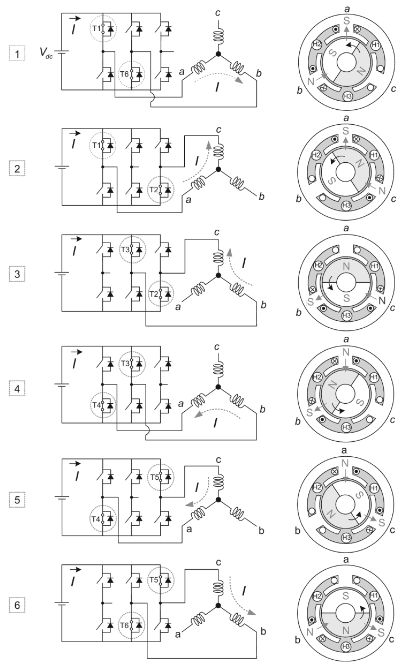
\includegraphics[width=11cm]{imagens/acionamento.png}
    \legendafonte{\cite{kim2017electric}.}
    \label{fig:sequencia-acionamento-bldc}
\end{figure}

 Nesta etapa de validação, a comutação opera em \textbf{malha aberta} (alinhamento e rampa forçada); a \textbf{transição para comutação em malha fechada orientada por ZCD} permanece como passo subsequente, após a confirmação da sequência 6-step e do condicionamento do sinal, conforme detalhado no Capítulo 4.

 Quando a aplicação necessita que o motor possua apenas uma velocidade, a fonte de alimentação de tensão fixa é suficiente. Para casos onde é necessário variar a velocidade do motor, a técnica de Modulação por Largura de Pulso (PWM) é normalmente empregada. Um ESC, por exemplo, utiliza PWM para ajustar a tensão média aplicada ao motor, controlando assim sua velocidade. Essa técnica, no entanto, pode demandar a utilização de controladores que comparem a velocidade desejada com a medida no rotor para um controle preciso, estratégia desenvolvida teoricamente na Seção~\ref{sec:controle_pi}. 

 \subsubsection{Análise da Ondulação de Torque (Torque Ripple)}
A principal desvantagem intrínseca à comutação forçada de seis passos (malha aberta) é a geração de uma ondulação de torque (\textit{torque ripple}), que se manifesta como pulsações no torque de saída do motor \cite{jahns1984torque, ali2017implementation}. Essas pulsações podem causar oscilações na velocidade, ruído acústico e vibrações mecânicas, sendo particularmente prejudiciais em aplicações que exigem alta precisão de movimento \cite{jahns1996pulsating}. A frequência desta ondulação é seis vezes a frequência elétrica fundamental do motor, correspondendo a uma pulsação a cada evento de comutação \cite{jahns1984torque}. Conforme analisado em trabalhos seminais como os de Jahns (1984) e Hendershot \& Miller (1994), este fenômeno é consequência de dois fatores principais \cite{kim2017electric, hendershot1994design}.

\begin{enumerate}
    \item \textbf{Incompatibilidade de Formas de Onda:} O modelo ideal do controle trapezoidal assume uma forma de onda de corrente perfeitamente retangular e uma FCEM perfeitamente trapezoidal. Na prática, a FCEM dos motores reais raramente é um trapézio ideal, e a corrente injetada não é perfeitamente retangular. Qualquer desalinhamento ou incompatibilidade entre a forma de onda da corrente e a da FCEM resulta em variações no torque produzido, conforme a equação $T_{e} = (e_{a} \cdot i_{a} + e_{b} \cdot i_{b} + e_{c} \cdot i_{c}) / \omega$ \cite{hendershot1994design}.

    \item \textbf{Transientes de Comutação:} A causa mais significativa da ondulação de torque é o próprio processo de comutação. Devido à indutância presente nos enrolamentos do motor, a corrente não pode variar instantaneamente. Quando o controlador comuta de um passo para o outro (por exemplo, de A-B para A-C), há um período de tempo finito durante o qual a corrente na fase que está sendo desligada (fase B) decai através do diodo de roda livre, e a corrente na fase que está sendo ligada (fase C) aumenta através da chave ativa \cite{jahns1996pulsating, joice2013compensation}. Durante este intervalo de comutação, o torque eletromagnético total produzido pelo motor não é constante. A taxa de variação da corrente na fase de entrada ($\frac{di_{in}}{dt}$) e na de saída ($\frac{di_{out}}{dt}$) é assimétrica devido à diferença de potencial aplicada em cada malha. Enquanto o crescimento da corrente na fase de entrada é retardado pela oposição da sua Força Contra-Eletromotriz (FCEM), o decaimento da corrente na fase de saída é acelerado pela soma da tensão do barramento com a sua respectiva FCEM durante a condução pelo diodo de roda livre. Essa diferença nas derivadas de corrente gera uma perturbação transitória na soma total das correntes do estator, resultando em um mergulho (\textit{dip}) ou pico de torque a cada $60^{\circ}$ elétricos \cite{choi1998commutation, chen2019commutation}.

\end{enumerate}

A ondulação de torque não é apenas um efeito colateral indesejado; é a manifestação mecânica de uma conversão de energia eletromecânica periodicamente de baixo rendimento. O objetivo do motor é converter potência elétrica em potência mecânica (torque vezes velocidade) de forma contínua e suave. Durante os intervalos de comutação, o vetor de corrente do estator está em transição entre duas posições estáveis. Neste período, o alinhamento entre o campo magnético do estator e o campo magnético do rotor desvia-se momentaneamente da orientação ótima de $90^{\circ}$ elétricos necessária para a produção máxima de torque. Consequentemente, para uma mesma magnitude de corrente de entrada, o torque de saída é reduzido, representando uma queda transitória no rendimento da conversão de energia. A ondulação de torque observada é, portanto, o resultado direto desses intervalos de conversão sub-ótima, inerentes à natureza discreta do chaveamento de seis passos.

\subsubsection{Modulação por Largura de Pulso (PWM)} 

O controle de velocidade e torque de motores BLDC exige a imposição de uma tensão terminal variável nos enrolamentos do estator. Dado que as fontes de alimentação primárias disponíveis na maioria das aplicações (como baterias e fontes de bancada) operam com uma tensão contínua fixa ($V_{DC}$), faz-se necessária a aplicação da técnica de Modulação por Largura de Pulso (PWM, \textit{Pulse Width Modulation}). Esta técnica consiste no chaveamento periódico de alta frequência dos semicondutores de potência da ponte inversora, aplicando pulsos de tensão retangulares de amplitude fixa e largura variável à carga indutiva.

O parâmetro fundamental que rege o comportamento do PWM é a razão cíclica (\textit{duty cycle}, $D$), definida matematicamente como a relação entre o tempo em que o sinal permanece em nível lógico alto ($t_{on}$) e o período total do ciclo de chaveamento ($T$), conforme expresso na Equação \ref{eq:duty_cycle}:

\begin{equation}
D = \frac{t_{on}}{T} = t_{on} \cdot f_c
\label{eq:duty_cycle}
\end{equation}

Em que $f_c$ representa a frequência de portadora ou frequência de chaveamento. A tensão média efetiva entregue aos enrolamentos do estator ($V_{m\text{é}dia}$) é obtida por meio da integração do sinal de tensão instantâneo ao longo de um período completo, resultando em uma relação linear direta com a razão cíclica, explicitada na Equação \ref{eq:v_media}:

\begin{equation}
V_{m\text{é}dia} = \frac{1}{T} \int_{0}^{t_{on}} V_{DC} \, dt = \frac{t_{on}}{T} V_{DC} = D \cdot V_{DC}
\label{eq:v_media}
\end{equation}

A seleção da frequência de chaveamento ($f_c$) constitui um compromisso crítico de projeto de engenharia, governado por restrições de ordem magnética, acústica e térmica. Motores BLDC de alto desempenho e tamanho reduzido comumente apresentam resistência estatórica e indutância de fase extremamente baixas. Sob frequências de chaveamento reduzidas, a baixa constante de tempo indutiva ($\tau = L/R$) resulta em uma elevada ondulação de corrente (\textit{current ripple}), o que culmina em perdas excessivas por efeito Joule no cobre e geração de ruído acústico na faixa audível humana (20 Hz a 20 kHz). 

Por outro lado, a elevação excessiva de $f_c$ acarreta o aumento linear das perdas por comutação (\textit{switching losses}) nos MOSFETs de potência, dadas pela transição periódica entre os estados de condução e bloqueio, conforme modelado simplificadamente na Equação \ref{eq:perdas_comutacao}:

\begin{equation}
P_{sw} = V_{DC} \cdot I_{out} \cdot f_c \cdot \left( \frac{t_r + t_f}{2} \right)
\label{eq:perdas_comutacao}
\end{equation}

Em que $I_{out}$ é a corrente de saída, e $t_r$ e $t_f$ são os tempos de subida (\textit{rise time}) e descida (\textit{fall time}) do transistor, respectivamente. No desenvolvimento de inversores voltados a protótipos de ESC, adota-se rotineiramente uma frequência de portadora de aproximadamente 20 kHz. Esse valor se posiciona no limiar superior da audição humana, mitigando poluição sonora decorrente do magnetostritismo, ao mesmo tempo em que preserva a integridade térmica dos transistores e minimiza a ondulação da corrente contínua através do estator.

No âmbito da comutação trapezoidal de seis passos, o sinal PWM gerado pelo periférico de controle (como o módulo MCPWM) pode ser aplicado de diferentes formas aos braços do inversor trifásico durante o setor de condução de $120^\circ$ elétricos. Destacam-se as seguintes estratégias de modulação unipolar:

\begin{itemize}
    \item \textbf{Estratégia H\_PWM - L\_ON:} O sinal PWM de alta frequência é aplicado exclusivamente ao transistor do lado da alta (\textit{High-Side}), enquanto o dispositivo correspondente do lado da baixa (\textit{Low-Side}) permanece permanentemente conduzindo em nível contínuo (SINK) durante todo o intervalo de $120^\circ$. Esta abordagem reduz sensivelmente as perdas por comutação totais da ponte, uma vez que apenas uma das chaves ativas sofre transições rápidas a cada período.
    \item \textbf{Estratégia H\_ON - L\_PWM:} Configuração inversa à anterior, na qual a chave superior é mantida saturada em nível lógico alto e a chave inferior modula a corrente em alta frequência.
\end{itemize}

Durante os períodos de desligamento do PWM ($t_{off}$) na estratégia H\_PWM - L\_ON, a energia armazenada no campo magnético indutivo da bobina força a circulação da corrente através do diodo de roda livre intrínseco do MOSFET complementar, estabelecendo um circuito de recirculação. A correta temporização e o entendimento de que a largura de pulso atua diretamente na magnetização do estator formam o alicerce para o controle de torque do sistema.

\begin{figure}[htbp]
    \centering
    \caption{Modulação por largura de pulso utilizando uma fonte de $100V$.}
    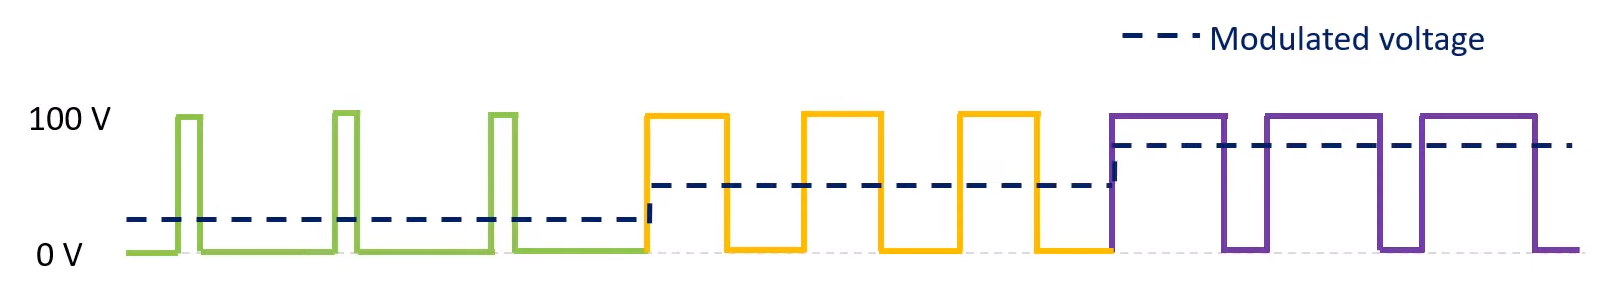
\includegraphics[width=0.85\textwidth]{imagens/PWM.png}
    \legendafonte{\cite{matlabBLDC}.}
    \label{fig:pwm-fonte-100v}
\end{figure}

 \subsection{Estratégia de Partida em Malha Aberta para Operação \textit{Sensorless}}

A implementação de um controle \textit{sensorless} eficaz depende da capacidade do controlador de estimar a posição do rotor a partir de grandezas elétricas, mais comumente a FCEM. Contudo, esta abordagem apresenta um desafio fundamental: em repouso (velocidade zero), não há movimento relativo entre os ímãs do rotor e os enrolamentos do estator, e, portanto, nenhuma FCEM é gerada \cite{ti2013sensorless, nxp2023sensorless}. Nesta condição "cega", o controlador não possui informações sobre a posição angular do rotor, tornando impossível determinar qual par de fases deve ser energizado para iniciar a rotação na direção desejada. Para superar essa limitação, é necessária uma rotina de partida especializada, operando em malha aberta, que força o motor a girar até que uma velocidade suficiente seja atingida para que a FCEM se torne detectável e o controle em malha fechada possa assumir. Este procedimento é universalmente dividido em duas fases sequenciais: alinhamento e comutação forçada.

\subsubsection{Alinhamento do Rotor}

O primeiro passo para uma partida confiável é estabelecer uma posição inicial conhecida para o rotor. A fase de alinhamento realiza isso ao energizar um conjunto específico de enrolamentos do estator com uma corrente contínua (DC) por um período de tempo pré-determinado \cite{ti2022minimizing, nxp2023sensorless}. Por exemplo, o controlador pode aplicar uma tensão positiva à fase C e conectar as fases A e B ao terra \cite{ti2022minimizing}. Esta ação cria um campo magnético estático e fixo no estator. Os ímãs permanentes do rotor, livres para girar, irão se alinhar com este campo para minimizar a relutância magnética do circuito, de forma análoga a uma agulha de bússola se alinhando com o campo magnético terrestre. Ao final deste processo, o rotor estará travado em uma posição angular conhecida e previsível. Os parâmetros críticos que governam esta fase são a duração do alinhamento e a magnitude da corrente de alinhamento \cite{ti2022minimizing}.

 A fase de alinhamento funciona como uma etapa de otimização pré-torque, o seu objetivo primordial é condicionar o sistema para que o primeiro passo de comutação dinâmica gere o máximo torque possível. O maior desafio ao iniciar um motor a partir do repouso é vencer a inércia da carga e o atrito estático, o que exige um impulso de torque inicial elevado. A teoria de motores elétricos, conforme estabelecido na Seção 1.1.1, dita que o torque é maximizado quando o campo magnético do estator está orientado a $90^{\circ}$ elétricos em relação ao campo do rotor. O algoritmo de controle é projetado sabendo a posição final do rotor após o alinhamento. Assim, a primeira combinação de fases a ser energizada na fase seguinte (rampa de aceleração) é escolhida para criar um novo vetor de campo magnético do estator que esteja precisamente na orientação ótima em relação à posição agora conhecida do rotor. Isso garante que o primeiro passo dinâmico produza um torque potente e eficaz, "chutando" o rotor para o movimento e superando as resistências iniciais. Uma duração de alinhamento insuficiente ou uma corrente muito baixa pode resultar em um alinhamento incompleto, levando a um torque inicial fraco e, consequentemente, a uma falha na partida \cite{ti2022minimizing}.

\subsubsection{Comutação Forçada (Rampa de Aceleração)}

Com o rotor devidamente alinhado, o controlador inicia a fase de comutação forçada. Nesta etapa, o sistema opera em malha aberta, comutando as fases em uma sequência predefinida, sem qualquer realimentação da posição do rotor \cite{nxp2023sensorless}. A frequência de comutação não é aplicada abruptamente; em vez disso, ela é aumentada gradualmente a partir de um valor inicial baixo, seguindo um perfil de aceleração pré-programado, conhecido como "curva de partida em malha aberta" (\textit{open-loop starting curve}) \cite{ti2022minimizing}. Esta rampa de aceleração é definida por coeficientes pré-definidos \cite{ti2022minimizing}.

Durante esta fase, o controlador essencialmente comanda a rotação do campo magnético do estator e "assume" que o rotor, devido à sua inércia e ao torque gerado, conseguirá acompanhar este campo giratório. O processo continua, com a frequência de comutação aumentando progressivamente, até que a velocidade de rotação do motor seja alta o suficiente (tipicamente em torno de $5\%$ da velocidade nominal) para que a FCEM gerada nos enrolamentos atinja uma amplitude que possa ser medida de forma confiável \cite{ti2022minimizing, nxp2023sensorless}. Neste ponto, o sistema realiza a transição (\textit{handoff}) do controle em malha aberta para um modo de controle em malha fechada (por exemplo, baseado na detecção de cruzamento por zero da FCEM), que é de maior rendimento e robusto para a operação contínua.

\subsection{Desafios e Limitações da Partida Forçada}

A estratégia de partida em malha aberta não é isenta de desafios e limitações significativas. A sua natureza "cega" a torna vulnerável a variações de carga e a parâmetros não ideais do sistema.

\subsubsection{Análise do Fenômeno de Perda de Sincronismo (Stall)}

O risco mais proeminente do controle em malha aberta é a perda de sincronismo, comumente conhecida como \textit{stall} ou perda de passo. Este fenômeno ocorre quando a aceleração real do rotor não consegue acompanhar a velocidade de rotação do campo magnético do estator imposta pelo controlador. Se o torque de carga aplicado ao eixo do motor, somado à sua própria inércia, for maior que o torque eletromagnético que o motor consegue produzir em um determinado passo, o rotor "perderá o passo" e ficará para trás \cite{nxp2023sensorless}. Isso pode ser causado por uma carga inicial muito elevada ou por uma rampa de aceleração excessivamente agressiva, que aumenta a frequência de comutação mais rápido do que o rotor consegue acelerar \cite{ti2022minimizing}.

Uma vez que o sincronismo é perdido, o alinhamento entre os campos do rotor e do estator se torna desfavorável, e a produção de torque efetivo colapsa. O resultado é um movimento errático, vibrações intensas, ruído audível e, frequentemente, a parada completa do motor, enquanto o controlador continua a injetar corrente nos enrolamentos de forma ineficaz. Este estado pode levar a picos de corrente perigosos para a eletrônica de potência. Por essa razão, o controle em malha aberta é inadequado para aplicações com cargas variáveis ou que exigem alto torque de partida.

\subsubsection{Outros Efeitos Adversos}

Além do risco de perda de passo, a partida forçada apresenta outras desvantagens:

\begin{itemize}
    \item \textbf{Picos de Corrente:} No início da partida, a velocidade do motor é baixa ou nula, o que significa que a FCEM, que normalmente se opõe à tensão de alimentação e limita a corrente, também é baixa ou inexistente. Sem essa oposição, a corrente que flui para os enrolamentos é limitada apenas pela resistência ôhmica e pela tensão aplicada, podendo atingir valores muito elevados se não for cuidadosamente controlada pelo \textit{duty cycle} do PWM. Estes picos de corrente podem estressar a bateria e os componentes da ponte inversora.
    \item \textbf{Vibração e Baixo Rendimento:} Como o controle é feito "às cegas", o alinhamento entre o campo do estator e o rotor durante a rampa de aceleração nunca é perfeito. Este desalinhamento constante é a fonte da ondulação de torque discutida anteriormente, que se manifesta como vibração mecânica e resulta em uma operação de baixo rendimento, onde uma parte da energia elétrica consumida é dissipada em vez de ser convertida em torque útil.
\end{itemize}

É fundamental reiterar que a partida forçada em malha aberta é uma fase transitória e um meio para um fim. É uma estratégia de \textit{bootstrap} projetada exclusivamente para levar o motor de um estado de repouso para uma velocidade operacional mínima, onde métodos de controle em malha fechada, de maior rendimento, precisos e robustos, podem ser ativados para a operação contínua do sistema \cite{ti2022minimizing, nxp2023sensorless}.

\section{Controle Proporcional-Integral em Malhas Fechadas de ESC}
\label{sec:controle_pi}

Além da comutação trapezoidal e da modulação PWM, a operação precisa de um ESC em regime depende de \textbf{malhas de realimentação} que ajustem continuamente a tensão média aplicada ao motor (ou a corrente de fase) de modo a acompanhar referências de corrente ou velocidade impostas pelo operador. Neste trabalho, essa função é desempenhada por controladores \textbf{proporcional-integral (PI)}, algoritmo amplamente adotado em acionamentos de motores BLDC e PMSM por combinar simplicidade de implementação, robustez frente a perturbações de carga e capacidade de eliminar erro estacionário \cite{krishnan2010permanent, xia2012permanent, kim2017electric}.

\subsection{Distinção entre Malhas de Comutação e Malhas PI}
\label{subsec:distincao_malhas}

Um ESC trifásico opera com \textbf{duas camadas de controle independentes}, que não devem ser confundidas. A primeira decide \textit{quando} comutar as fases (sincronismo angular com o rotor); a segunda decide \textit{quanto} esforço elétrico aplicar em cada passo (corrente ou velocidade desejada). A nomenclatura ``malha aberta'' e ``malha fechada'' aplica-se separadamente a cada camada, e não ao sistema como um todo.

\begin{table}[htbp]
\centering
\caption{Duas camadas de controle no ESC deste trabalho}
\label{tab:camadas_controle}
\resizebox{\textwidth}{!}{%
\begin{tabular}{p{3.2cm}p{4.8cm}p{3.2cm}p{3.8cm}}
\toprule
\textbf{Camada} & \textbf{Grandeza regulada} & \textbf{Realimentação} & \textbf{Estado neste projeto} \\
\midrule
Comutação 6-step & Instante de troca de fase (posição do rotor) & FCEM/ZCD ou temporizador & Malha \textbf{aberta} na validação atual (rampa por temporizador; ver Subseções anteriores deste capítulo) \\
Malha PI & Corrente de fase e/ou velocidade & INA240 + ADC1; intervalo entre passos & Malha \textbf{fechada} sempre que o PI está ativo \\
\bottomrule
\end{tabular}%
}
\legendafonte{Elaborado pelo autor (2026).}
\end{table}

Três esclarecimentos estruturam o uso desses termos ao longo deste trabalho:

\begin{enumerate}
    \item \textbf{O controlador PI é malha fechada, e não aberta.} Por definição, o PI exige comparar referência $r$ com medição $y$ (Equação~\ref{eq:pi_continuo} adiante). No firmware, a corrente de fase é medida pelos amplificadores INA240 e convertida pelo ADC1; no modo velocidade, a velocidade é estimada a partir do intervalo entre passos de comutação. Sem essa realimentação, não haveria erro $e = r - y$ nem termo integral, tratar-se-ia apenas de um \textit{duty cycle} fixo ou de uma rampa pré-programada, o que não caracteriza um regulador PI.
    \item \textbf{O sistema ESC como um todo não é inteiramente malha fechada.} Na fase de validação descrita neste trabalho, a comutação trapezoidal avança em \textbf{malha aberta}: a sequência 6-step progride por temporizador (rampa de frequência elétrica), sem usar o cruzamento por zero da FCEM para sincronizar o rotor. A infraestrutura de \textit{hardware} para comutação em malha fechada por ZCD (comparadores LM339, neutro virtual) está projetada, mas o \textit{handover} para essa modalidade permanece como etapa subsequente (Subseção anterior sobre comutação \textit{sensorless} e Capítulo de Resultados). Enquanto isso, as malhas PI de corrente e velocidade operam em paralelo, em malha fechada, regulando o esforço elétrico dentro de cada passo comutado.
    \item \textbf{Onde cada conceito é tratado neste texto.} A comutação e a partida em malha aberta alinhamento, rampa forçada, risco de \textit{stall} e transição futura para ZCD, são desenvolvidas na Seção anterior (Controlador Eletrônico de Velocidade). A presente seção trata exclusivamente das malhas PI em malha fechada (corrente e velocidade). A implementação no firmware, ganhos $K_p$ e $K_i$, e os resultados de bancada encontram-se nos Capítulos de Metodologia e de Resultados e Discussão.
\end{enumerate}

\subsection{Fundamentos do Controlador PI}

Em uma malha fechada, o controlador recebe uma \textbf{referência} $r$ (por exemplo, corrente ou velocidade desejada) e compara-a com a \textbf{medição} $y$ proveniente dos sensores. O \textbf{erro} instantâneo é definido como:
\begin{equation}
    e(t) = r - y(t)
\end{equation}
A ação de controle $u(t)$ combina uma resposta proporcional ao erro atual e uma resposta integral que acumula o erro ao longo do tempo:
\begin{equation}
    u(t) = K_p \, e(t) + K_i \int_0^t e(\tau) \, d\tau
    \label{eq:pi_continuo}
\end{equation}
onde $K_p$ é o ganho proporcional e $K_i$ o ganho integral. O termo proporcional confere resposta imediata a desvios; o termo integral corrige desvios persistentes, pois continua a agir enquanto $e(t) \neq 0$.

Em sistemas embarcados, a Equação~\ref{eq:pi_continuo} é implementada em tempo discreto com período de amostragem $T_s = \Delta t$. Adotando integração de Euler, a forma recorrente adotada neste projeto é:
\begin{equation}
    P_k = K_p \, e_k
    \label{eq:pi_p_discreto}
\end{equation}
\begin{equation}
    I_k = I_{k-1} + K_i \, e_k \, \Delta t
    \label{eq:pi_i_discreto}
\end{equation}
\begin{equation}
    u_k = \mathrm{clamp}(P_k + I_k,\; u_{min},\; u_{max})
    \label{eq:pi_saida}
\end{equation}
Quando a saída $u_k$ atinge os limites físicos do atuador (por exemplo, o teto de \textit{duty cycle} do PWM), o integrador pode continuar a acumular erro (\textit{windup}), provocando sobressinal ao sair da saturação. Por isso, impõe-se \textbf{anti-windup} por limitação (\textit{clamping}) do estado integral $I_k$ dentro de intervalos $[I_{min}, I_{max}]$, detalhes de implementação no firmware são apresentados nos Capítulos de Metodologia e de Resultados.

\subsection{Limitações do Controle Proporcional Puro}

Um controlador puramente proporcional ($u = K_p \cdot e$) reage instantaneamente ao erro, mas apresenta uma limitação estrutural: na presença de perturbações constantes ou de plantas com comportamento integrador, o sistema estabiliza com \textbf{erro estacionário} não nulo. Intuitivamente, um ganho $K_p$ finito exige um erro residual para produzir a ação de controle necessária ao equilíbrio.

No contexto de um ESC trapezoidal, essa limitação manifesta-se de forma concreta. Para manter uma corrente de fase constante $I_{cmd}$, o \textit{duty cycle} do PWM deve compensar não apenas a queda ôhmica nos enrolamentos, mas também a FCEM, cujo valor cresce linearmente com a velocidade ($e_a = K_e \cdot \omega$). À medida que o motor acelera ou a tensão do barramento decai, o duty necessário para o mesmo $I_{cmd}$ aumenta. Um controlador P puro, com ganho fixo, não possui mecanismo para ajustar esse \textit{offset} operacional: a corrente medida estabilizaria abaixo da referência. O termo integral supre exatamente essa lacuna, acumulando a ação necessária até anular o erro residual.

De forma análoga, na regulagem de velocidade, variações de carga mecânica (atrito, inércia da carga) exigem correntes distintas para manter a mesma velocidade. Sem integral, um controlador P de velocidade deixaria um desvio permanente entre a referência e a rotação medida sempre que a carga se alterasse.

\subsection{Exclusão do Termo Derivativo: por que PI e não PID}

O controlador PID acrescenta um termo derivativo $K_d \cdot de/dt$, sensível à taxa de variação do erro. Embora possa melhorar a resposta transitória em plantas bem modeladas e pouco ruidosas, a inclusão do termo D neste ESC traz desvantagens que superam os benefícios esperados:

\begin{itemize}
    \item \textbf{Amplificação de ruído:} A corrente de fase é medida por amplificadores INA240 e convertida pelo ADC1 a $1\,\text{kHz}$, em ambiente de comutação PWM a $20\,\text{kHz}$ e de sequência trapezoidal de seis passos. O termo derivativo amplificaria as componentes de alta frequência (ripple de corrente, transientes de comutação), degradando a qualidade do sinal de realimentação e podendo induzir oscilações na saída do controlador.
    \item \textbf{Dinâmica dominante lenta:} A malha externa de velocidade e a sequência de comutação operam em escala de milissegundos (frequência elétrica de dezenas a centenas de hertz). A dinâmica mecânica e elétrica do sistema trapezoidal não se beneficia de previsão agressiva baseada em derivadas, ao contrário de malhas de corrente de FOC em dezenas de quilohertz.
    \item \textbf{Derivative kick:} Degraus na referência (comando do operador via gatilho analógico) produzem picos instantâneos em $de/dt$. Embora o firmware limite a taxa de variação da referência (\textit{slew rate limiter}), o termo D permaneceria sensível a saltos residuais de erro.
    \item \textbf{Prática consolidada:} Malhas de corrente e de velocidade em acionamentos BLDC trapezoidais utilizam PI como padrão industrial \cite{krishnan2010permanent, xia2012permanent, hanselman2003brushless}. A sintonia de três ganhos ($K_p$, $K_i$, $K_d$) com filtragem do termo derivativo agregaria complexidade sem retorno mensurável na arquitetura de controle adotada neste trabalho.
\end{itemize}

Por essas razões, o firmware deste projeto implementa estritamente controladores PI, sem termo derivativo.

\subsection{Aplicabilidade ao ESC Trifásico Deste Trabalho}

A estratégia de controle PI adapta-se diretamente à topologia do ESC desenvolvido, organizada em uma ou duas malhas conforme o modo operacional:

\begin{itemize}
    \item \textbf{Malha interna de corrente:} O PI de corrente compara a referência $I_{cmd}$ (limitada pelo operador ou pela malha externa) com a corrente de fase medida e produz o \textit{duty cycle} do PWM (0 a 95\,\%). Essa malha regula o esforço elétrico do motor, aproximando torque $\propto I$, e constitui a primeira linha de defesa contra sobrecorrente antes das proteções analógicas e de software.
    \item \textbf{Malha externa de velocidade (modo cascata):} Quando habilitado o modo de controle por velocidade, um segundo PI compara $RPM_{cmd}$ com a velocidade estimada a partir do intervalo entre passos de comutação 6-step e gera a referência de corrente para o PI interno. A corrente adapta-se automaticamente à carga mecânica, dentro do limite de 5\,A configurado.
    \item \textbf{Modo corrente direta:} Com apenas o PI de corrente ativo, a velocidade resultante depende da carga e da rampa de comutação em malha aberta, útil para ensaios de bancada com esforço elétrico limitado.
\end{itemize}

Dois requisitos de implementação derivam diretamente da teoria PI e condicionam o firmware: (1) o período de amostragem $\Delta t = 1\,\text{ms}$ deve ser estável, pois o termo integral da Equação~\ref{eq:pi_i_discreto} depende de $\Delta t$ constante, requisito tratado na Seção~\ref{sec:fundamentos_software}; (2) a saturação da saída em 95\,\% de \textit{duty cycle}, imposta pela recarga do capacitor de \textit{bootstrap} dos drivers IR2110, torna obrigatório o anti-windup para evitar sobressinal ao retornar da saturação.

A materialização dessas malhas no firmware, arquitetura em cascata, ganhos $K_p$ e $K_i$, temporizador de 1\,kHz e validação em bancada, é descrita no Capítulo de Metodologia e discutida no Capítulo de Resultados e Discussão.

\section{Aspectos de Eletrônica de Potência}

A implementação física do inversor exige a compreensão de componentes e técnicas que viabilizam a comutação em alta frequência e corrente.

\subsection{O MOSFET de Potência e Perdas}
O MOSFET (\textit{Metal-Oxide-Semiconductor Field-Effect Transistor}) é o dispositivo de chaveamento predominante em aplicações de baixa e média tensão devido à sua alta velocidade de comutação e facilidade de acionamento \cite{rashid2014power}. Em um inversor para controle de motores, o MOSFET não atua na região linear (amplificação), mas alterna entre os estados de corte (chave aberta) e saturação (chave fechada).

O rendimento do inversor é limitado por dois mecanismos principais de perda no MOSFET \cite{kim2017electric}:
\begin{itemize}
    \item \textbf{Perdas por Condução ($P_{cond}$):} Quando o transistor está ligado, ele apresenta uma resistência interna residual entre dreno e fonte, denominada $R_{DS(on)}$. A potência dissipada é dada por $P_{cond} = I_{D}^2 \cdot R_{DS(on)}$. Componentes modernos buscam minimizar o $R_{DS(on)}$ para reduzir o aquecimento.
    \item \textbf{Perdas por Comutação ($P_{sw}$):} Ocorrem durante a transição entre ligado e desligado. Como a tensão e a corrente não variam instantaneamente, há um breve período em que ambas são não-nulas, gerando um pico de potência dissipada. Esta perda é diretamente proporcional à frequência de chaveamento ($f_{sw}$) e à carga total de gate ($Q_g$) que o driver deve fornecer \cite{rashid2014power}.
\end{itemize}

\subsection{Seleção da Frequência de Chaveamento PWM}
\label{subsec:freq_chaveamento_pwm}

A frequência de chaveamento ($f_{sw}$) do PWM que modula os MOSFETs da ponte inversora é um parâmetro de projeto que acopla diretamente os mecanismos de perda descritos acima (em particular, $P_{sw} \propto f_{sw}$) à ondulação de corrente (\textit{ripple}) nas bobinas do motor e ao ruído acústico gerado por magnetostrição no estator \cite{mohan2003, hanselman2003brushless}. Não existe um valor universalmente ótimo: a indústria opera em faixas distintas conforme a aplicação, a dissipação térmica disponível no inversor e a carga de gate ($Q_g$) dos semicondutores selecionados \cite{rashid2014power}.

Neste trabalho adota-se \textbf{20 kHz} como compromisso de engenharia para o par MOSFET/driver IRFS7530--IR2110: a carga de gate elevada dos transistores automotivos selecionados torna inviável, com dissipação passiva no volume da placa, as faixas de alta performance do aeromodelismo (48 kHz ou 96 kHz, comuns em ESCs \textit{racing}), enquanto valores inferiores a 16 kHz reintroduziriam ruído audível. O dimensionamento quantitativo, perdas de comutação, \textit{ripple} de corrente e corrente média de \textit{gate} do driver, encontra-se na Subseção de Determinação da Frequência de Chaveamento do Capítulo de Metodologia.

\begin{table}[htbp]
    \centering
    \caption{Panorama de frequências de chaveamento PWM em acionamentos BLDC e afins}
    \label{tab:panorama_fsw_industria}
    \resizebox{\textwidth}{!}{%
    \begin{tabular}{lll}
    \toprule
    \textbf{Faixa típica} & \textbf{Segmento / aplicação} & \textbf{Característica principal} \\
    \midrule
    4--8 kHz & Drives industriais legados, ESCs de baixo custo & Audível; menores perdas de comutação \\
    8--12 kHz & Ferramentas elétricas, ESCs \textit{entry-level} & Zumbido perceptível ao operador \\
    16--24 kHz & ESCs BLDC genéricos, VANTs & Próximo ao limiar ultrassônico ($\approx 20\,\text{kHz}$) \\
    \textbf{20 kHz} & \textbf{Este projeto} & Equilíbrio térmico, silêncio e \textit{ripple} (Cap.~Metodologia) \\
    32--48 kHz & Aeromodelismo, \textit{drones} de consumo & Menor \textit{ripple}; $P_{sw}$ maior \\
    48--96 kHz & ESCs \textit{racing} (ex.: BLHeli, SimonK) & Alta resposta; exige baixo $Q_g$ e dissipação agressiva \\
    10--20 kHz+ & FOC industrial & Malha de corrente rápida; escopo distinto do trapezoidal 6-step \\
    \bottomrule
    \end{tabular}%
    }
    \legendafonte{Elaborado pelo autor (2026), com base em \cite{rashid2014power, hanselman2003brushless, mohan2003}.}
    \end{table}

\subsection{O Barramento DC e a Indutância Parasita}

Em inversores de fonte de tensão (VSI) que operam com altas frequências de chaveamento, a impedância da fonte de alimentação não pode ser considerada ideal. Os cabos de conexão entre a bateria e o inversor introduzem uma indutância parasita ($L_{par}$) significativa no circuito. Durante a comutação dos transistores, a rápida variação de corrente ($di/dt$) interage com essa indutância, gerando picos de tensão ($V_{spike}$) de acordo com a lei de Faraday-Lenz:

\begin{equation}
    V_{spike} = L_{par} \cdot \frac{di}{dt}
\end{equation}

Se não mitigados, esses picos podem superar a tensão de ruptura dos semicondutores, causando falhas catastróficas. Para solucionar esse problema, utiliza-se um banco de capacitores no barramento DC (\textit{DC Link}), posicionado fisicamente próximo aos interruptores. Este banco atua como uma fonte de tensão de baixa impedância local, fornecendo a corrente pulsada exigida pelo inversor e absorvendo a energia regenerada, além de filtrar a componente alternada (ripple) da corrente \cite{rashid2014power}.

Embora o cálculo analítico da capacitância mínima ($C_{min}$) seja classicamente derivado da máxima variação de tensão admissível ($\Delta V$) no barramento, conforme a Equação \ref{eq:cap_calc}:

\begin{equation}
    C_{min} = \frac{I_{peak} \cdot D \cdot (1-D)}{f_{sw} \cdot \Delta V}
    \label{eq:cap_calc}
\end{equation}

\noindent onde $f_{sw}$ é a frequência de chaveamento e $D$ é o ciclo de trabalho (\textit{Duty Cycle}) do inversor. Observa-se que o esforço máximo sobre o capacitor ocorre quando $D=0,5$, ponto em que o produto $D \cdot (1-D)$ é máximo.

Entretanto, em aplicações de baixa tensão e alta corrente (como em VANTs), o fator limitante do projeto não é apenas a armazenagem de carga ($C_{min}$), mas sim a capacidade de condução de corrente de ripple ($I_{Ripple,RMS}$) e a dissipação térmica. Capacitores eletrolíticos comerciais apresentam uma correlação inversa entre capacitância nominal e Resistência Série Equivalente (ESR).

Consequentemente, adota-se na prática de engenharia o sobredimensionamento do valor de capacitância (regras empíricas da ordem de $10\mu F$ a $20\mu F$ por Ampere de corrente de fase). Esta abordagem visa, primariamente, reduzir a ESR total do banco de capacitores através da associação paralela e do uso de encapsulamentos maiores, garantindo que a corrente eficaz drenada pelo inversor não exceda o \textit{Ripple Current Rating} dos componentes, prevenindo a degradação dielétrica prematura por superaquecimento \cite{rashid2014power}.

\subsection{Técnica de \textit{Bootstrap} para Acionamento \textit{High-Side}}
Em uma ponte inversora trifásica, os transistores do "lado alto" (\textit{High-Side}) têm seus drenos conectados ao barramento positivo ($V_{CC}$) e suas fontes conectadas às fases do motor. Para ligar um MOSFET Canal-N nesta posição, a tensão no \textit{gate} deve ser superior à tensão da fonte ($V_{GS} > V_{th}$). Contudo, quando o transistor liga, a tensão da fonte sobe para aproximadamente $V_{CC}$, exigindo que a tensão do \textit{gate} seja elevada para $V_{CC} + V_{drv}$.

A técnica de \textit{Bootstrap} é a solução mais comum e econômica para gerar essa tensão flutuante. Ela utiliza um capacitor ($C_{boot}$) e um diodo ($D_{boot}$). O princípio de operação é cíclico:
\begin{enumerate}
    \item Quando o transistor do "lado baixo" (\textit{Low-Side}) está ligado, o terminal da fase é aterrado. O capacitor $C_{boot}$ é então carregado através do diodo pela fonte de alimentação auxiliar ($V_{drv}$).
    \item Quando o \textit{Low-Side} desliga e o \textit{High-Side} precisa ser acionado, a carga armazenada em $C_{boot}$ atua como uma "bateria flutuante", fornecendo a corrente necessária para carregar o \textit{gate} do transistor superior.
\end{enumerate}

\textbf{Limitação Importante:} O circuito de \textit{Bootstrap} não permite operação com ciclo de trabalho (\textit{duty cycle}) de 100\% indefinidamente. O transistor \textit{Low-Side} deve ser ligado periodicamente para recarregar o capacitor. Se o capacitor descarregar por falta de comutação, a tensão $V_{GS}$ cai, podendo levar o MOSFET superior a operar na região linear e falhar por superaquecimento.

\subsubsection{Dimensionamento do Capacitor de Bootstrap}

O capacitor de \textit{bootstrap} ($C_{boot}$), embora fisicamente conectado ao circuito do driver, tem como função primária atuar como um reservatório de energia flutuante para alimentar a porta (\textit{gate}) do MOSFET superior \cite{infineonAN978}. O driver atua apenas como a chave de transferência, drenando carga de $C_{boot}$ e injetando-a na capacitância de entrada do MOSFET para promover sua saturação.

Consequentemente, o dimensionamento deste capacitor depende intrinsecamente da quantidade de carga que o MOSFET exige para ligar, parâmetro conhecido como Carga Total de Gate ($Q_g$). A carga total ($Q_{tot}$) demandada do capacitor a cada ciclo de comutação é composta pela carga do MOSFET somada às perdas internas do driver \cite{infineonAN978}:

\begin{equation}
    Q_{tot} = \underbrace{Q_g}_{\text{Carga do MOSFET}} + \underbrace{(I_{qbs} + I_{leak}) \cdot T_{on}}_{\text{Consumo do Driver e Fugas}}
\end{equation}

\noindent onde $I_{qbs}$ é a corrente quiescente do estágio de alta do driver e $I_{leak}$ representa as correntes de fuga. Como $Q_g$ é tipicamente muito maior que o consumo do driver em frequências usuais, ele é o fator determinante no dimensionamento. Para garantir que a tensão no capacitor não sofra uma queda brusca ($\Delta V_{boot}$) ao transferir essa carga para o MOSFET o que poderia reduzir a tensão $V_{GS}$ abaixo do nível seguro de saturação, a capacitância mínima é calculada como \cite{infineonAN978}:

\begin{equation}
    C_{boot} \geq \frac{Q_{tot}}{\Delta V_{boot}}
\end{equation}

Na prática de engenharia, para assegurar robustez contra transitórios e variações de temperatura, adota-se um capacitor capaz de armazenar pelo menos 15 vezes a carga do gate do MOSFET ($Q_g$), garantindo uma fonte de tensão rígida para o driver \cite{adamsDT98}.

\section{Fundamentos de Software para Sistemas de Controle Embarcado}
\label{sec:fundamentos_software}

O hardware de potência de um ESC constituído pela ponte inversora, os \textit{drivers} de \textit{gate} e os sensores de corrente é condição necessária, mas não suficiente, para o funcionamento do sistema. Sem um firmware estruturado que orquestre com precisão a sequência de comutação, as malhas de controle e as rotinas de proteção, o hardware é inerte. Esta seção apresenta conceitos gerais de engenharia de software embarcado que fundamentam as decisões de projeto do firmware desenvolvido neste trabalho.

\subsection{Camada de Abstração de Hardware (HAL)}

Um microcontrolador moderno como o ESP32 é, do ponto de vista do programador, uma coleção de periféricos configuráveis por registradores de memória: o módulo MCPWM gera sinais PWM quando seus registradores de período, \textit{duty cycle} e \textit{dead-time} são programados; o ADC converte tensão em código binário quando seu registrador de controle é acionado; o GPIO muda de estado quando um bit específico é escrito em um endereço de memória mapeada.

Escrever a lógica de controle do motor diretamente em termos desses registradores cria um acoplamento rígido entre o algoritmo e o silício: uma mudança de pino, a substituição do amplificador de corrente ou a migração para outro microcontrolador exigiria reescrever o código de controle integralmente. A solução consiste em interpor uma \textbf{Camada de Abstração de Hardware} (\textit{Hardware Abstraction Layer}  HAL), uma fronteira de software que encapsula todo o acesso físico ao periférico e expõe uma interface de funções simples e independente de hardware.

A analogia mais imediata é o conceito de \textbf{interface padronizada}. Assim como uma tomada normalizada permite conectar qualquer equipamento certificado independentemente da fiação interna da instalação elétrica, a HAL permite que o algoritmo de controle se ``conecte'' ao hardware por meio de chamadas como \texttt{hal\_adc\_read\_mv(channel)} ou \texttt{hal\_pwm\_set\_phase\_conduction(phase, mode)}, sem conhecer os registradores subjacentes. A implementação dessas funções, os detalhes da "fiação interna", está confinada aos módulos da HAL.

O fluxo de dependência resultante é \textbf{unidirecional}: camadas superiores invocam camadas inferiores, mas o inverso nunca ocorre. O controlador PI, por exemplo, processa exclusivamente grandezas numéricas em ponto flutuante (referência, medição e limites) sem incluir nenhum cabeçalho de periférico. Sua lógica matemática permanece idêntica independentemente de o sinal de corrente provir de um amplificador com \textit{shunt} resistivo de $1\,m\Omega$ ou de qualquer outro sensor. A conversão de milivolts para ampères, específica de cada componente, fica restrita ao módulo de \textit{driver} correspondente, imediatamente acima da HAL e abaixo do controlador. Essa separação garante que a calibração de um sensor, a troca de um CI ou a alteração de um pino implique a modificação de exatamente um módulo, sem risco de regressão em qualquer outro subsistema.

\subsection{Máquinas de Estado Finito (FSM) em Sistemas Críticos}

O controle de um ESC envolve condições operacionais mutuamente exclusivas: o motor não pode estar simultaneamente em aceleração e em estado de falha; o PWM não deve ser armado quando a tensão da bateria está abaixo do mínimo seguro; a sequência de comutação trapezoidal só pode começar após o alinhamento estático do rotor. Gerenciar essas restrições por meio de combinações de variáveis booleanas dispersas pelo código torna o sistema propenso a inconsistências: um único caminho de execução imprevisto pode resultar em duas dessas variáveis assumindo valores contraditórios simultaneamente, com consequências potencialmente catastróficas para a eletrônica de potência.

A solução formal para esse problema é a \textbf{Máquina de Estados Finita} (\textit{Finite State Machine} FSM), um modelo computacional em que o sistema ocupa, em qualquer instante, exatamente um entre um conjunto discreto e pré-definido de estados, e transita entre eles por regras explícitas e condicionadas. A FSM elimina estados ilegais por construção: se os estados definidos são \texttt{IDLE}, \texttt{RUNNING} e \texttt{FAULT}, é estruturalmente impossível para o sistema estar em \texttt{RUNNING} e \texttt{FAULT} simultaneamente. A saída é sempre determinística, não há estado intermediário ou flutuante entre 0 e 1. Uma FSM de software estende esse conceito para múltiplos estados e múltiplas condições de transição, com a mesma propriedade de determinismo. Assim o projetista de firmware garante que transições de estado proibidas jamais sejam ativadas, por meio das condições de guarda programadas nas funções de transição.

Em sistemas de potência, as vantagens da FSM são diretas:

\begin{itemize}
    \item \textbf{Segurança estrutural:} transições perigosas são proibidas por código. A função de arme do ESC verifica explicitamente a ausência de subtensão e de falha ativa antes de liberar o PWM. Um sistema baseado em \textit{flags} poderia armar inadvertidamente caso uma dessas verificações fosse omitida em algum caminho de execução.
    \item \textbf{Rastreabilidade:} o estado atual é uma variável enumerada (\textit{enum}) visível na telemetria serial e na dashboard Wi-Fi, facilitando o diagnóstico em bancada sem necessidade de osciloscópio ou depurador em circuito.
    \item \textbf{Resposta a falhas centralizada:} qualquer fonte de erro seja de hardware analógico, interrupção de sobrecorrente ou supervisão de software, converge para uma única função de entrada em falha, que executa a sequência de desligamento em ordem determinística: primeiro os \textit{drivers} de potência, depois o PWM, garantindo que o estágio de potência esteja seguro mesmo que operações subsequentes falhem.
    \item \textbf{Manutenibilidade:} novas condições de transição por exemplo, uma proteção térmica futura são adicionadas à FSM sem modificar a lógica de comutação ou a camada de entrada, isolando o impacto da mudança em um único módulo.
\end{itemize}

Além da FSM do ESC, sistemas embarcados de controle de motores frequentemente empregam \textbf{sub-máquinas de estado} aninhadas. A sequência de partida de um motor \textit{sensorless} (alinhamento estático, comutação forçada em rampa e transição para malha fechada) é ela própria uma FSM interna, cujos estados e transições são independentes da FSM de nível superior e executam apenas quando esta autoriza a operação.

\subsection{Programação Orientada ao Tempo Real: Interrupções e Concorrência}

Um ESC opera com múltiplas cadências temporais simultâneas e de magnitudes muito diferentes: a proteção de sobrecorrente deve agir em microssegundos para evitar a destruição dos semicondutores; a malha de controle de corrente deve amostrar e calcular a cada milissegundo para manter a estabilidade dinâmica; a interface com o operador pode ser atualizada a cada dezenas de milissegundos sem comprometer o desempenho. Atender a todos esses requisitos em um único fluxo sequencial de programa é inviável.

A solução combina dois mecanismos complementares. O primeiro é a \textbf{rotina de serviço de interrupção} (\textit{Interrupt Service Routine} ISR), uma função que o hardware dispara automaticamente em resposta a um evento externo, a borda de descida de um sinal de falha, o cruzamento por zero de uma tensão, interrompendo o programa principal e executando com latência mínima. Por analogia com circuitos analógicos, a ISR é o equivalente funcional de um \textbf{comparador de janela}: quando o sinal monitorado cruza o limiar, uma ação imediata é disparada, independentemente de qualquer outra atividade do sistema. Para garantir baixa latência e segurança, ISRs devem executar apenas o mínimo indispensável: desarmar o PWM, sinalizar o evento por uma variável de estado e retornar ao fluxo principal. Operações mais elaboradas, como imprimir diagnóstico na serial ou calcular médias de corrente, são executadas no contexto do programa principal, que consulta a variável de sinalização periodicamente, padrão denominado \textit{deferred processing} (processamento diferido).

O segundo mecanismo é o \textbf{temporizador periódico de hardware}, que dispara um \textit{callback} em intervalos fixos e precisos, independentemente da duração de outras operações em andamento. A malha de controle de um ESC deve ser amostrada a período exatamente constante para que a equação do integrador $I_k = I_{k-1} + K_i \cdot e_k \cdot \Delta t$ (Equação~\ref{eq:pi_i_discreto}, Seção~\ref{sec:controle_pi}) produza resultados matematicamente corretos: qualquer variação em $\Delta t$ introduz erro sistemático na integral e pode desestabilizar a malha fechada. Temporizadores de \textit{software} que dependem do loop principal acumulam variação de tempo (\textit{jitter}) inevitável, causada por operações de duração variável como transmissão Bluetooth e formatação de \textit{strings}; o temporizador de hardware garante período estável e determinístico, requisito essencial para a integridade da malha de controle.

A coexistência de ISRs, temporizadores e loop principal introduz o problema de \textbf{concorrência}: uma variável escrita pela ISR pode ser lida pelo loop principal em estado inconsistente se o compilador, em sua otimização, armazenar o valor em um registrador da CPU em vez de na memória. O qualificador \textbf{\texttt{volatile}}, aplicado a essas variáveis compartilhadas, instrui o compilador a sempre ler o valor diretamente da memória, garantindo a coerência dos dados entre contextos de execução concorrentes.

\section{Estado da Arte em Algoritmos de Controle e Estimação}
\label{sec:estado_da_arte}

Embora a técnica de comutação trapezoidal com detecção de cruzamento por zero (ZCD) seja robusta e amplamente utilizada, o desenvolvimento de microcontroladores de alto desempenho e FPGAs permitiu a implementação de estratégias de controle mais sofisticadas. Estas técnicas visam superar as limitações do ZCD, principalmente em baixas velocidades e no controle de torque.

\subsection{Métodos Baseados em Força Contraeletromotriz (FCEM)}
Esta categoria, na qual se insere a técnica utilizada neste trabalho, fundamenta-se na proporcionalidade entre a tensão induzida e a velocidade angular do rotor.
\begin{itemize}
    \item \textbf{Detecção de Cruzamento por Zero (ZCD):} Monitora a tensão na fase não energizada para determinar os instantes de comutação. É simples e eficaz para médias e altas rotações.
    \item \textbf{Integração da FCEM:} Em vez de buscar apenas o zero, integra-se a área sob a curva da tensão induzida. Isso oferece maior imunidade a ruídos de PWM (ruído de comutação), pois a integração atua como um filtro natural.
    \item \textbf{Limitação e Solução:} A principal dificuldade é a inexistência de sinal em velocidade zero ou muito baixa. A solução padrão da indústria é a "Comutação Forçada" (\textit{Sensorless Trapezoidal Control}), onde aplica-se uma sequência cega inicial para arrancar o motor até que a FCEM seja detectável.
\end{itemize}

\subsection{Controle Orientado de Campo (FOC) e Observadores}
O Controle Orientado de Campo (\textit{Field-Oriented Control} - FOC) representa o padrão de alto desempenho. Diferente do controle trapezoidal que aciona o motor em passos discretos, o FOC controla as correntes do estator para manter o vetor de campo magnético sempre ortogonal ao rotor (90 graus), maximizando o torque por ampere e reduzindo a ondulação de torque. Para operação sem sensores (\textit{sensorless}), utilizam-se observadores matemáticos:

\begin{itemize}
    \item \textbf{Observadores de Estado (Luenberger):} Utilizam as equações diferenciais do motor para estimar a corrente e a FCEM. A diferença entre a corrente estimada e a medida (erro) é usada para corrigir a estimativa da posição do rotor em tempo real.
    \item \textbf{Filtro de Kalman Estendido (EKF):} Uma abordagem estocástica que considera as incertezas do modelo e o ruído das medições. O EKF prediz o estado futuro do sistema e corrige a predição com base nas medições atuais, sendo extremamente robusto em ambientes ruidosos, embora exija alto poder computacional.
    \item \textbf{Observadores Adaptativos:} Ajustam dinamicamente os parâmetros do modelo (como resistência ou fluxo) durante a operação, compensando variações térmicas que poderiam degradar a precisão da estimativa.
\end{itemize}

\subsection{Técnicas Baseadas em Análise de Sinais e Harmônicos}
Existem métodos que exploram as não-linearidades e características construtivas do motor para inferir a posição, úteis especialmente em baixa velocidade onde a FCEM é nula.
\begin{itemize}
    \item \textbf{Detecção de Ondulação de Corrente (\textit{Current Ripple}):} A interação entre os polos do rotor e as ranhuras do estator gera pequenas ondulações na corrente. Algoritmos de processamento de sinal podem contar essas ondulações para estimar a velocidade e posição.
    \item \textbf{Método de Injeção de Alta Frequência:} Aplica-se um sinal de tensão de alta frequência e baixa amplitude. Devido à saliência magnética do rotor ($L_d \neq L_q$), a resposta de corrente varia conforme a posição angular, permitindo detectar a posição mesmo com o motor parado.
\end{itemize}

\section{Parâmetros Críticos para Modelagem Dinâmica}
\label{sec:parametros_modelagem}

A implementação de algoritmos avançados, como o FOC e os Observadores de Estado, exige um conhecimento preciso dos parâmetros intrínsecos do motor. A precisão do modelo matemático, e consequentemente a qualidade do controle, depende diretamente da caracterização das seguintes grandezas:

\begin{description}
    \item[Resistência de Estator ($R_s$):] Determina a queda de tensão ôhmica nos enrolamentos. Erros na identificação de $R_s$ causam desvios na estimativa de fluxo em baixas velocidades.
    
    \item[Indutância de Estator ($L_s, L_d, L_q$):] Fundamental para determinar a resposta dinâmica da corrente. Em motores de ímãs interiores (IPM), a diferença entre a indutância de eixo direto ($L_d$) e em quadratura ($L_q$) é o que permite o torque de relutância e a detecção de posição por injeção de sinal.
    
    \item[Fluxo do Rotor ($\lambda_m$):] Representa o fluxo magnético gerado pelos ímãs permanentes. É crucial para o cálculo do torque eletromagnético ($T_e$) e da constante de FCEM ($K_e$). Variações de temperatura podem alterar $\lambda_m$ (desmagnetização temporária), afetando a constante $K_T$ do motor.
    
    \item[Momento de Inércia ($J$) e Atrito ($B$):] Parâmetros mecânicos que ditam a resposta de velocidade do sistema. O conhecimento de $J$ é vital para o projeto das malhas de controle de velocidade, influenciando os ganhos $K_p$ e $K_i$ do controlador PI (Seção~\ref{sec:controle_pi}).
    
    \item[Número de Polos ($P$):] Define a relação entre a frequência elétrica e a velocidade mecânica. Um erro neste parâmetro inviabiliza qualquer algoritmo de estimação de velocidade.
\end{description}

O levantamento desses parâmetros geralmente requer equipamentos de precisão ou rotinas de auto-comissionamento implementadas no próprio inversor, destacando a complexidade superior dessas técnicas em comparação à comutação trapezoidal \textit{sensorless} por ZCD prevista neste projeto.


 \section{Vantagens e Desvantagens no uso de motores BLDC} 
 Os motores sem escovas, ou BLDC, apresentam diversas vantagens que contribuem para seu destaque em várias aplicações. O rendimento é uma característica proeminente, uma vez que convertem com maior rendimento a energia elétrica em torque quando comparados aos motores com escovas. Isso implica em uma demanda menor de energia para gerar a mesma quantidade de torque, resultando em um melhor desempenho global. A durabilidade é significativamente aprimorada, visto que a vida útil estendida desses motores está relacionada à ausência das escovas, componentes propensos a desgaste em motores convencionais. 

 Os motores de indução trifásicos (MIT) são concorrentes diretos dos motores BLDC, sendo que ambos são amplamente utilizados em diversas aplicações, cada uma com suas características distintas e vantagens específicas. Os motores de indução trifásicos são conhecidos pela sua confiabilidade, simplicidade de construção e custo relativamente baixo, quando comparado aos BLDC, utilizando os princípios da indução eletromagnética para gerar o torque e velocidade necessários para a aplicação. Embora tenham menor custo de produção quando comparados com os motores BLDC e podem ser controlados utilizando os mesmos protocolos, os MITs tendem a ter uma densidade de potência e torque menor em comparação com os motores BLDC, principalmente em baixas velocidades, o que pode ser uma consideração importante em aplicações que requerem alta potência em um espaço limitado. No entanto, os MITs apresentam melhor rendimento em operações de baixo torque, o que pode ser relevante em aplicações de mobilidade, como em veículos elétricos. 

 Os motores BLDC são conhecidos por seu rendimento energético superior, controle preciso de velocidade e torque, além de uma vida útil mais longa devido à ausência de escovas mecânicas \cite{gieras2009permanent}. Embora os BLDCs tenham um custo inicial mais elevado em comparação com os MITs, eles oferecem uma operação de maior rendimento, especialmente em condições de carga variável e velocidade ajustável. 

 Em resumo, os motores sem escovas oferecem um conjunto de vantagens notáveis, incluindo rendimento aprimorado, operação mais silenciosa, maior durabilidade e menor necessidade de manutenção. Contudo, esses benefícios vêm com um custo inicial mais elevado e a exigência de um controlador de velocidade, o que pode tornar sua implementação menos acessível em certos contextos. A escolha entre motores com escovas e sem escovas dependerá das prioridades específicas de uma aplicação, considerando tanto os benefícios quanto as limitações de cada tecnologia. 

 \section{Aplicações} 
 Os motores BLDC são amplamente utilizados em diversas aplicações devido às suas características únicas, como elevado rendimento, alta densidade de potência, baixo ruído, baixa manutenção e longa vida útil. Esses motores são preferidos em aplicações que necessitam de controle preciso de torque com oscilações inferiores em comparação com outros motores. 

 Uma das principais aplicações dos motores BLDC é em veículos elétricos, como carros, motocicletas, bicicletas e \textit{scooters} \cite{chau2007emerging}. Com o aumento da demanda por veículos elétricos, espera-se que os motores com tecnologia derivada do BLDC desempenhem um papel vital na indústria automotiva. Esses motores são usados para acionar o sistema de propulsão do veículo, fornecendo torque e potência para as rodas. Eles são preferidos em veículos elétricos devido à seu alta rendimento, baixo ruído e baixa manutenção. Essas motores são usados em aplicações que exigem alta precisão, controle de velocidade e torque, e baixo ruído.

